\appendix
\renewcommand\thefigure{\thesection.\arabic{figure}}
\renewcommand\thetable{\thesection.\arabic{table}}

\setcounter{figure}{0}
\setcounter{table}{0}

\section{Appendix}

\subsection{Income by Mexican State}

\begin{table}[p]
\centering
\begin{tabular}{>{\bfseries}l c c c}
\toprule
\multirow{2}{*}{State} & \multirow{2}{*}{Count in dataset} & Average Income & Average Income \\
& & (current dataset) & (Mexico's census) \\
\midrule
Aguascalientes & & & \\
Baja California Norte & & & \\
Baja California Sur & & & \\
Campeche & & & \\
Chiapas & & & \\
Chihuahua & & & \\
Ciudad de México & & & \\
Coahuila & & & \\
Colima & & & \\
Durango & & & \\
Estado de México & & & \\
Guanajuato & & & \\
Guerrero & & & \\
Hidalgo & & & \\
Jalisco & & & \\
Michoacan & & & \\
Morelos & & & \\
Nayarit & & & \\
Nuevo Leon & & & \\
Oaxaca & & & \\
Puebla & & & \\
Queretaro & & & \\
Quintana Roo & & & \\
San Luis Potosi & & & \\
Sinaloa & & & \\
Sonora & & & \\
Tabasco & & & \\
Tamaulipas & & & \\
Tlaxcala & & & \\
Veracruz & & & \\
Yucatan & & & \\
Zacatecas & & & \\
\bottomrule
\end{tabular}
\caption{Income information about Mexico's States \todo{Better Description}}
\label{tab:regions}
\end{table}

\subsection{Bayesian Metrics taking only users with calls in both directions}
\setcounter{topnumber}{8}
\setcounter{bottomnumber}{8}
\setcounter{totalnumber}{8}

\begin{figure}[p]
\centering
\begin{subfigure}[t]{\textwidth}
	\centering
	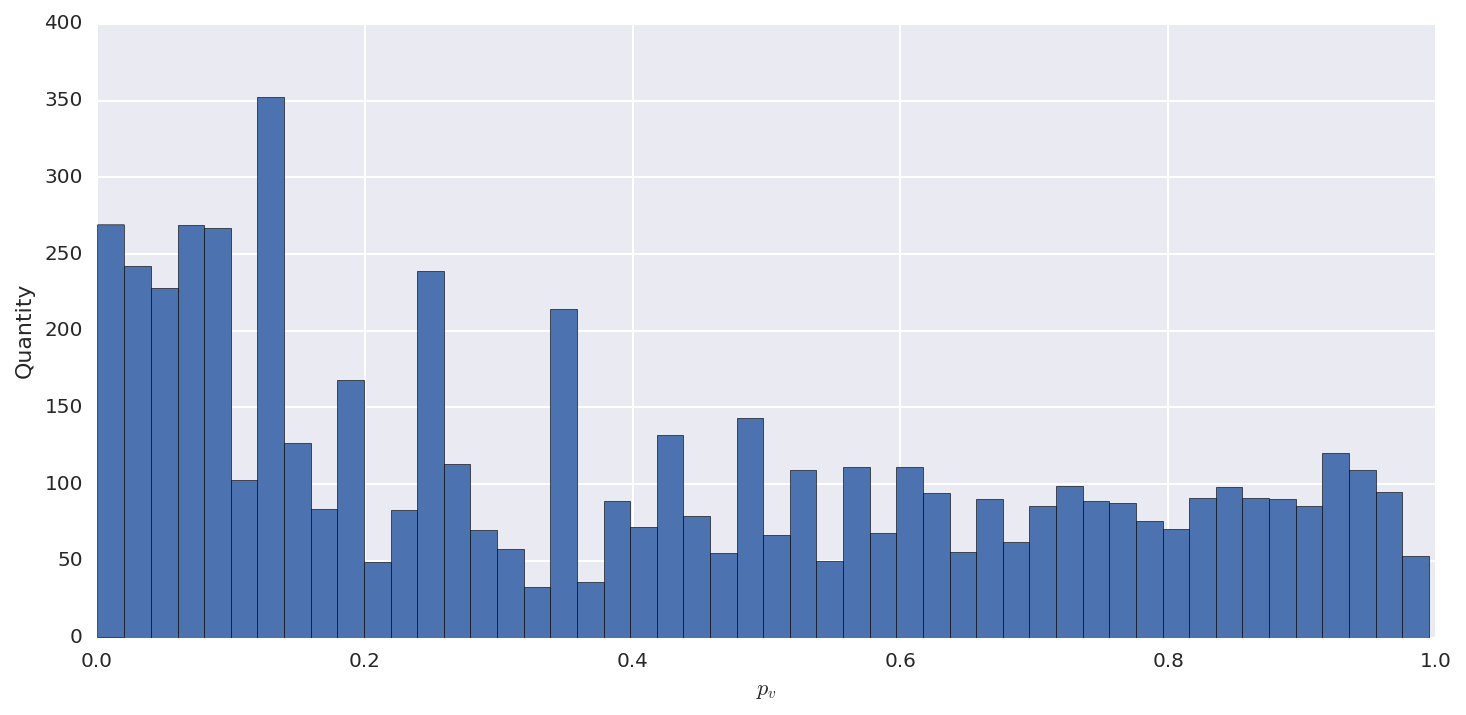
\includegraphics[height=.20\textheight]{figures/bayes/least1/hist_calls.png}
\end{subfigure}
\begin{subfigure}[b]{.49\textwidth}
	\raggedleft{}
	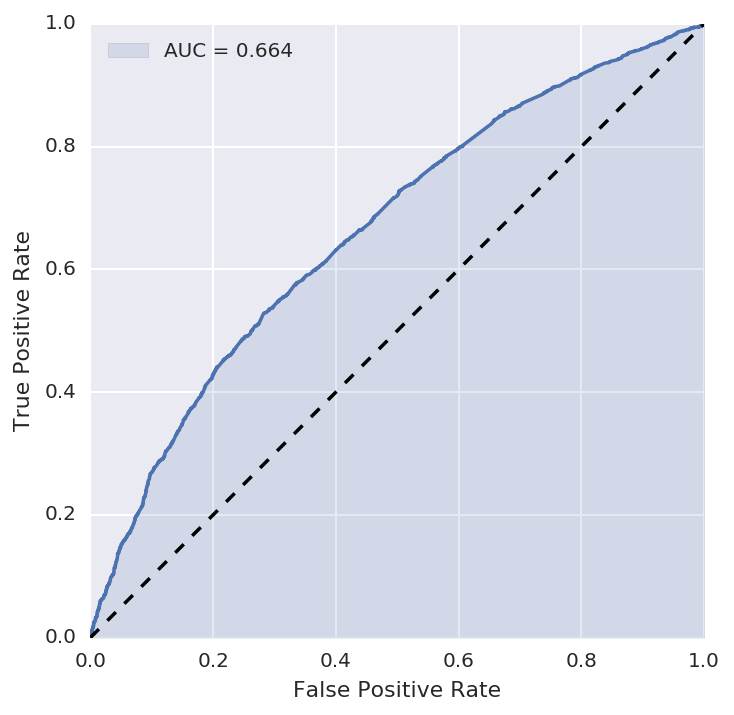
\includegraphics[height=.20\textheight]{figures/bayes/least1/roc_calls.png}
\end{subfigure}
\begin{subfigure}[b]{.49\textwidth}
	\raggedright{}
	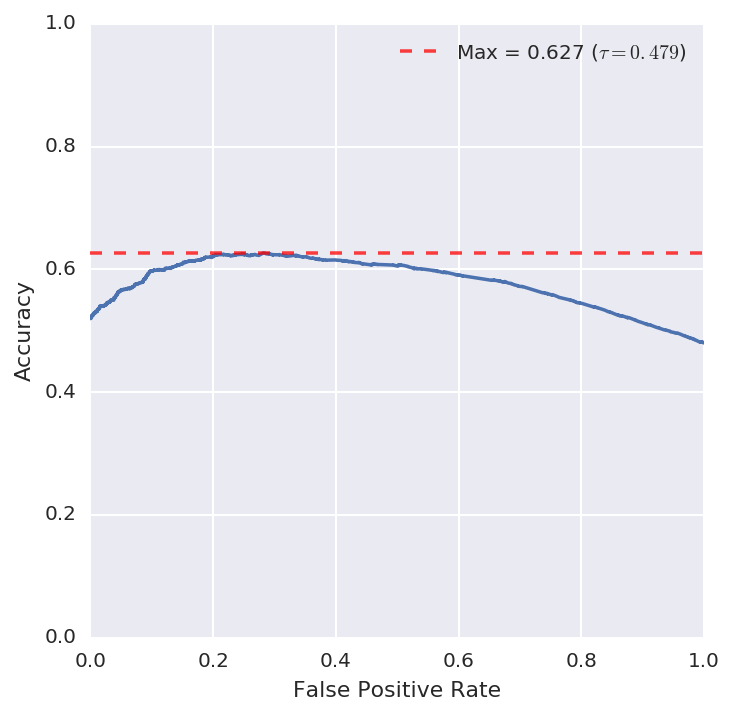
\includegraphics[height=.20\textheight]{figures/bayes/least1/accuracy_calls.png}
\end{subfigure}
\caption{Results for $\varpi = \calls$ when using $\hat{\Upsilon}^{\calls}$ instead of the whole set.}
\end{figure}

\begin{figure}[p]
\centering
\begin{subfigure}[t]{\textwidth}
	\centering
	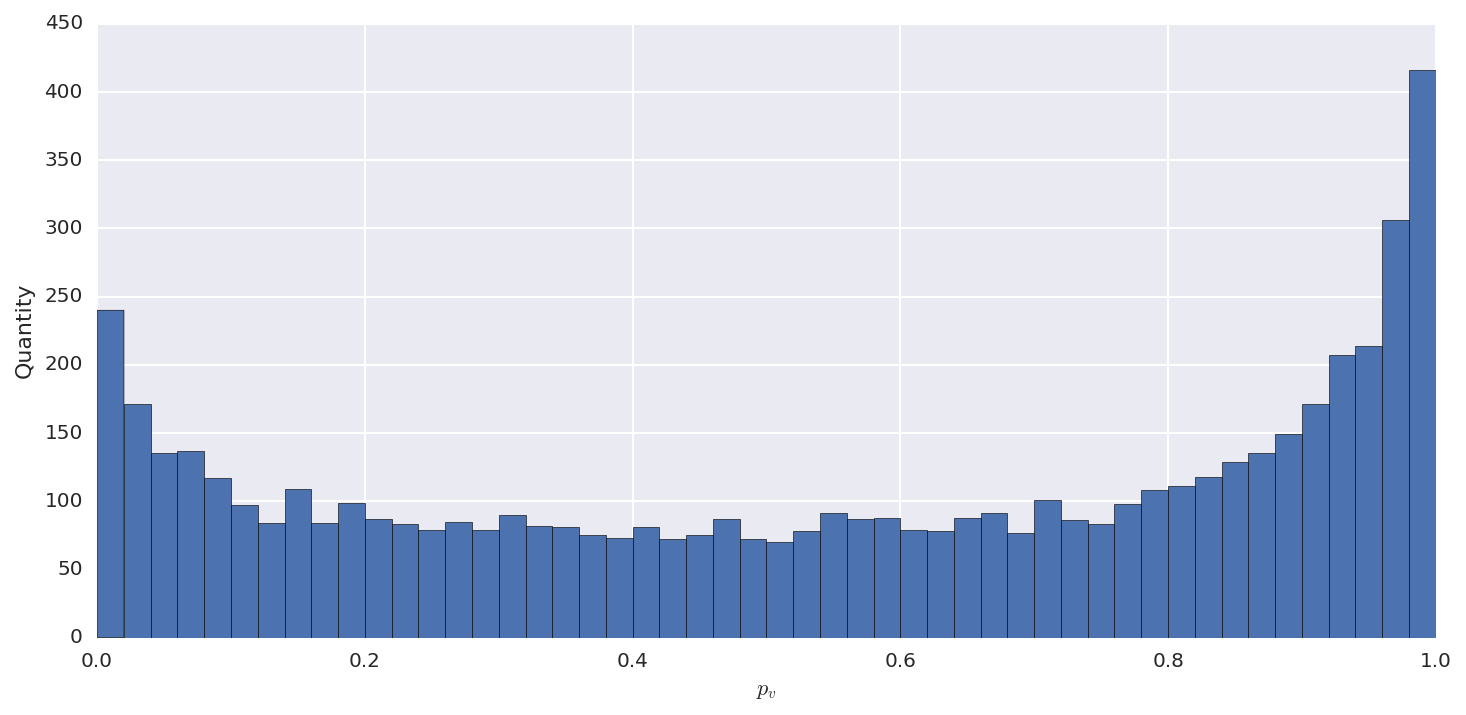
\includegraphics[height=.20\textheight]{figures/bayes/least1/hist_time.png}
\end{subfigure}
\begin{subfigure}[b]{.49\textwidth}
	\raggedleft{}
	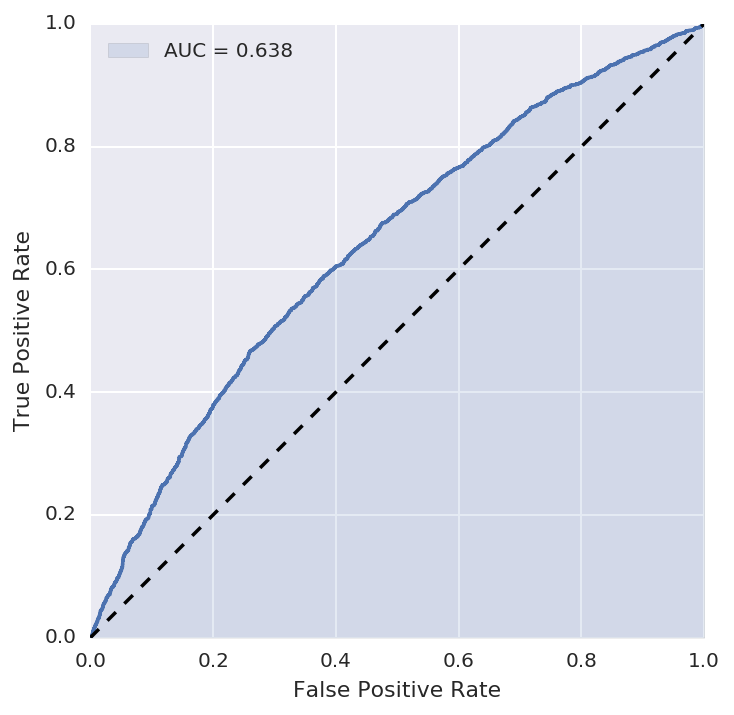
\includegraphics[height=.20\textheight]{figures/bayes/least1/roc_time.png}
\end{subfigure}
\begin{subfigure}[b]{.49\textwidth}
	\raggedright{}
	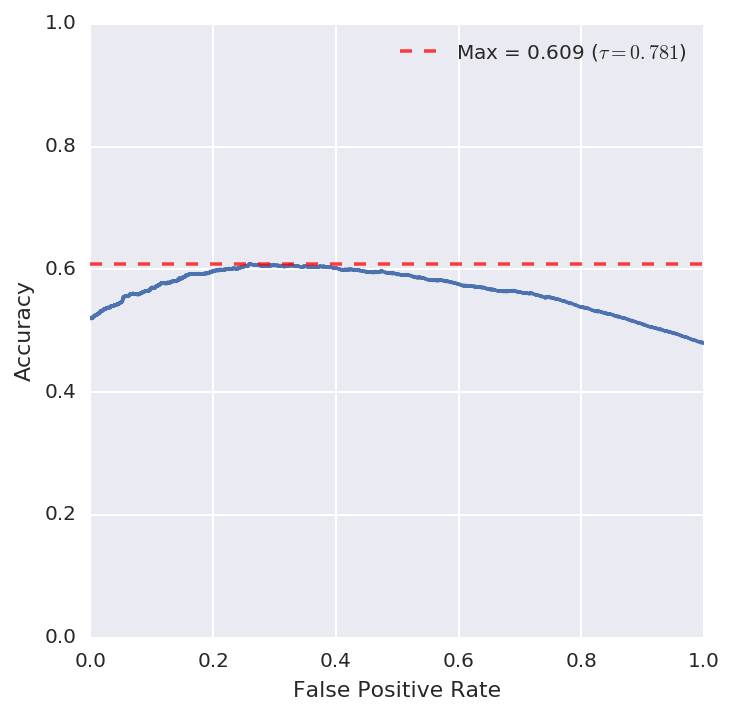
\includegraphics[height=.20\textheight]{figures/bayes/least1/accuracy_time.png}
\end{subfigure}
\caption{Results for $\varpi = \etime$ when using $\hat{\Upsilon}^{\calls}$ instead of the whole set. While the histogram is a lot more equitative than the one in Section~\ref{subsec:time_infer}, there are still the peaks at both ends are still distinguishable.}
\label{fig:time_infer_positive}
\end{figure}

\begin{figure}[p]
\centering
\begin{subfigure}[t]{\textwidth}
	\centering
	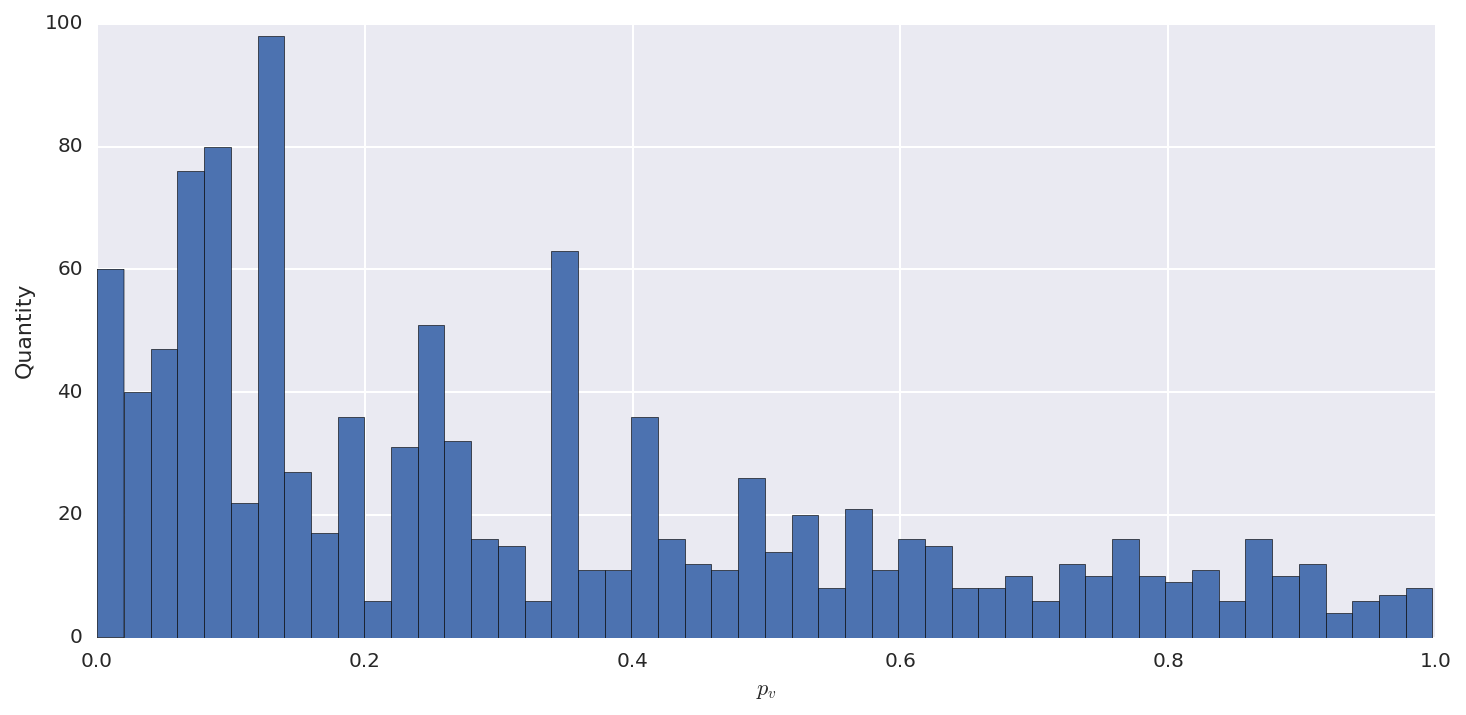
\includegraphics[height=.20\textheight]{figures/bayes/least1/hist_sms.png}
\end{subfigure}
\begin{subfigure}[b]{.49\textwidth}
	\raggedleft{}
	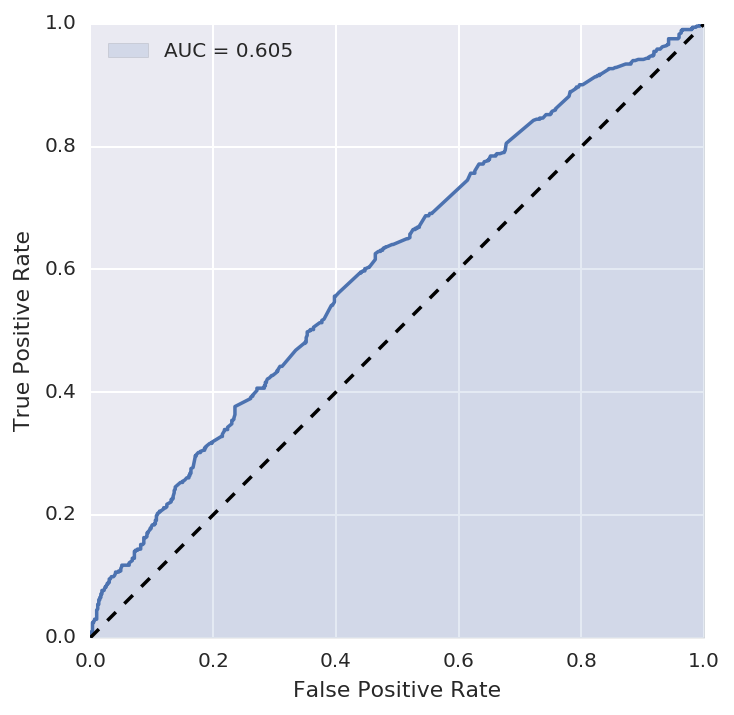
\includegraphics[height=.20\textheight]{figures/bayes/least1/roc_sms.png}
\end{subfigure}
\begin{subfigure}[b]{.49\textwidth}
	\raggedright{}
	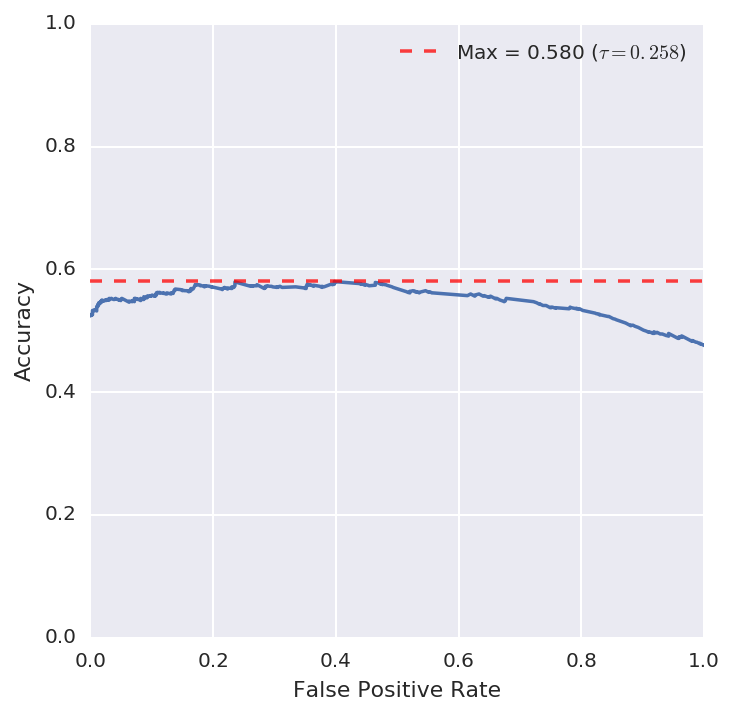
\includegraphics[height=.20\textheight]{figures/bayes/least1/accuracy_sms.png}
\end{subfigure}
\caption{Results for $\varpi = \sms$ when using $\hat{\Upsilon}^{\sms}$ instead of the whole set. As in the previous set, removing all cases where $\alpha = 1 \lor \beta = 1$ results in a more equitative histogram.}
\end{figure}

\begin{figure}[p]
\centering
\begin{subfigure}[t]{\textwidth}
	\centering
	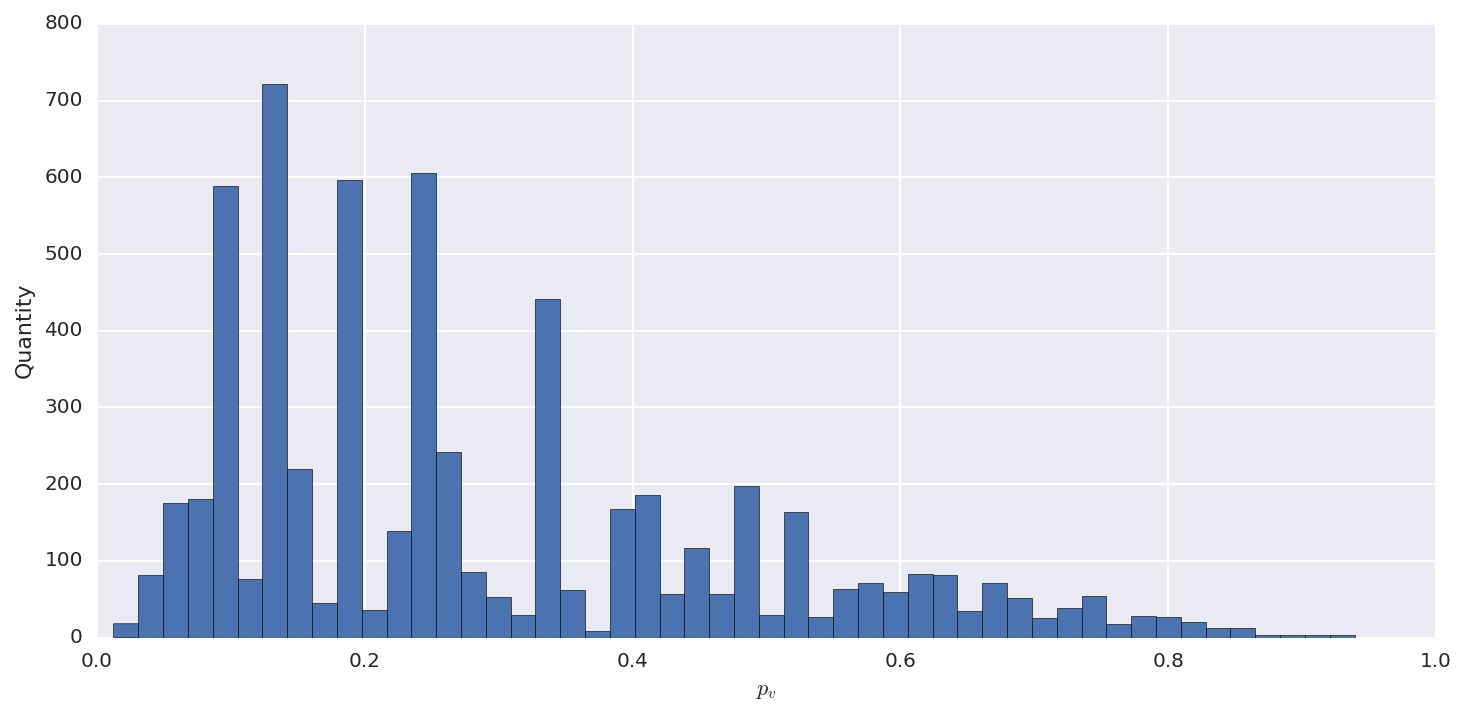
\includegraphics[height=.20\textheight]{figures/bayes/least1/hist_contacts.png}
\end{subfigure}
\begin{subfigure}[b]{.49\textwidth}
	\raggedleft{}
	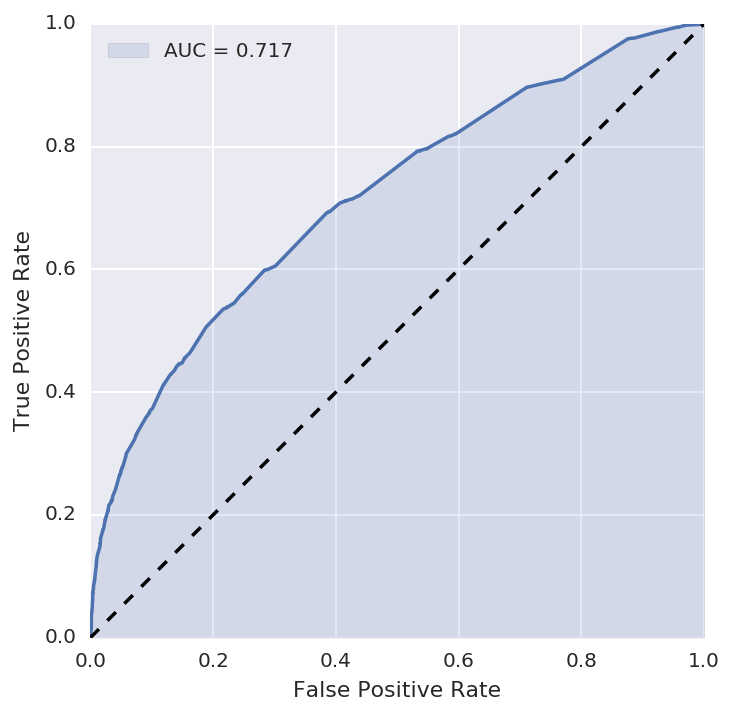
\includegraphics[height=.20\textheight]{figures/bayes/least1/roc_contacts.png}
\end{subfigure}
\begin{subfigure}[b]{.49\textwidth}
	\raggedright{}
	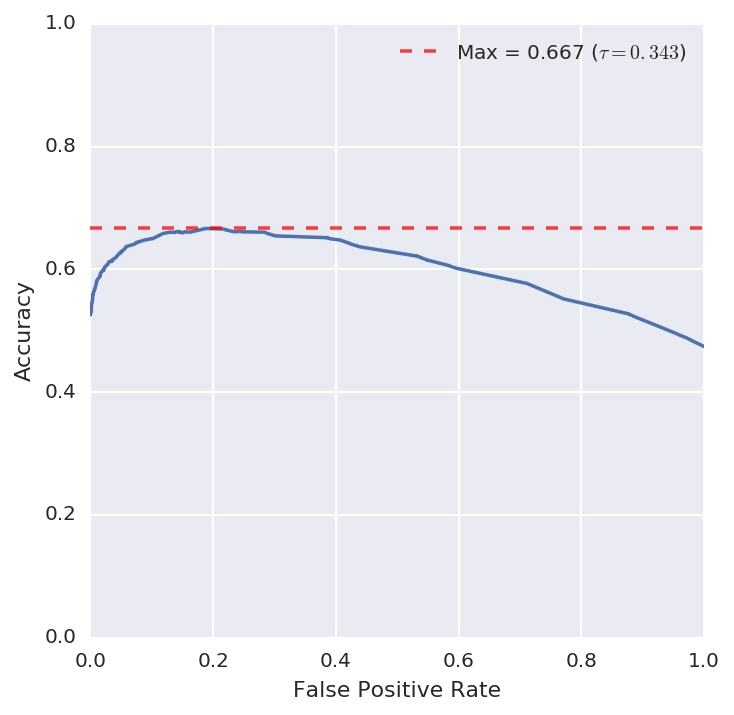
\includegraphics[height=.20\textheight]{figures/bayes/least1/accuracy_contacts.png}
\end{subfigure}
\caption{Results for $\varpi = \contacts$ when using $\hat{\Upsilon}$ instead of the whole set. Peaks are still visible due to the fact that it's easier to cluster users with the \emph{Socioeconomic Index} of their contacts.}
\end{figure}
